\documentclass[tikz,border=3mm]{standalone}
% Shared TikZ defaults
\usepackage{tikz}
\usetikzlibrary{arrows.meta,positioning,shapes.geometric}

% font and stroke defaults
\tikzset{
    every node/.style={font=\sffamily},
    line/.style={-Latex, thin},
    process/.style={rectangle, rounded corners, draw, thin, align=center, minimum width=36mm, minimum height=8mm},
    decision/.style={diamond, draw, thin, aspect=2.0, align=center, inner sep=1.5pt}
}

\usetikzlibrary{fit,backgrounds,calc}

\begin{document}
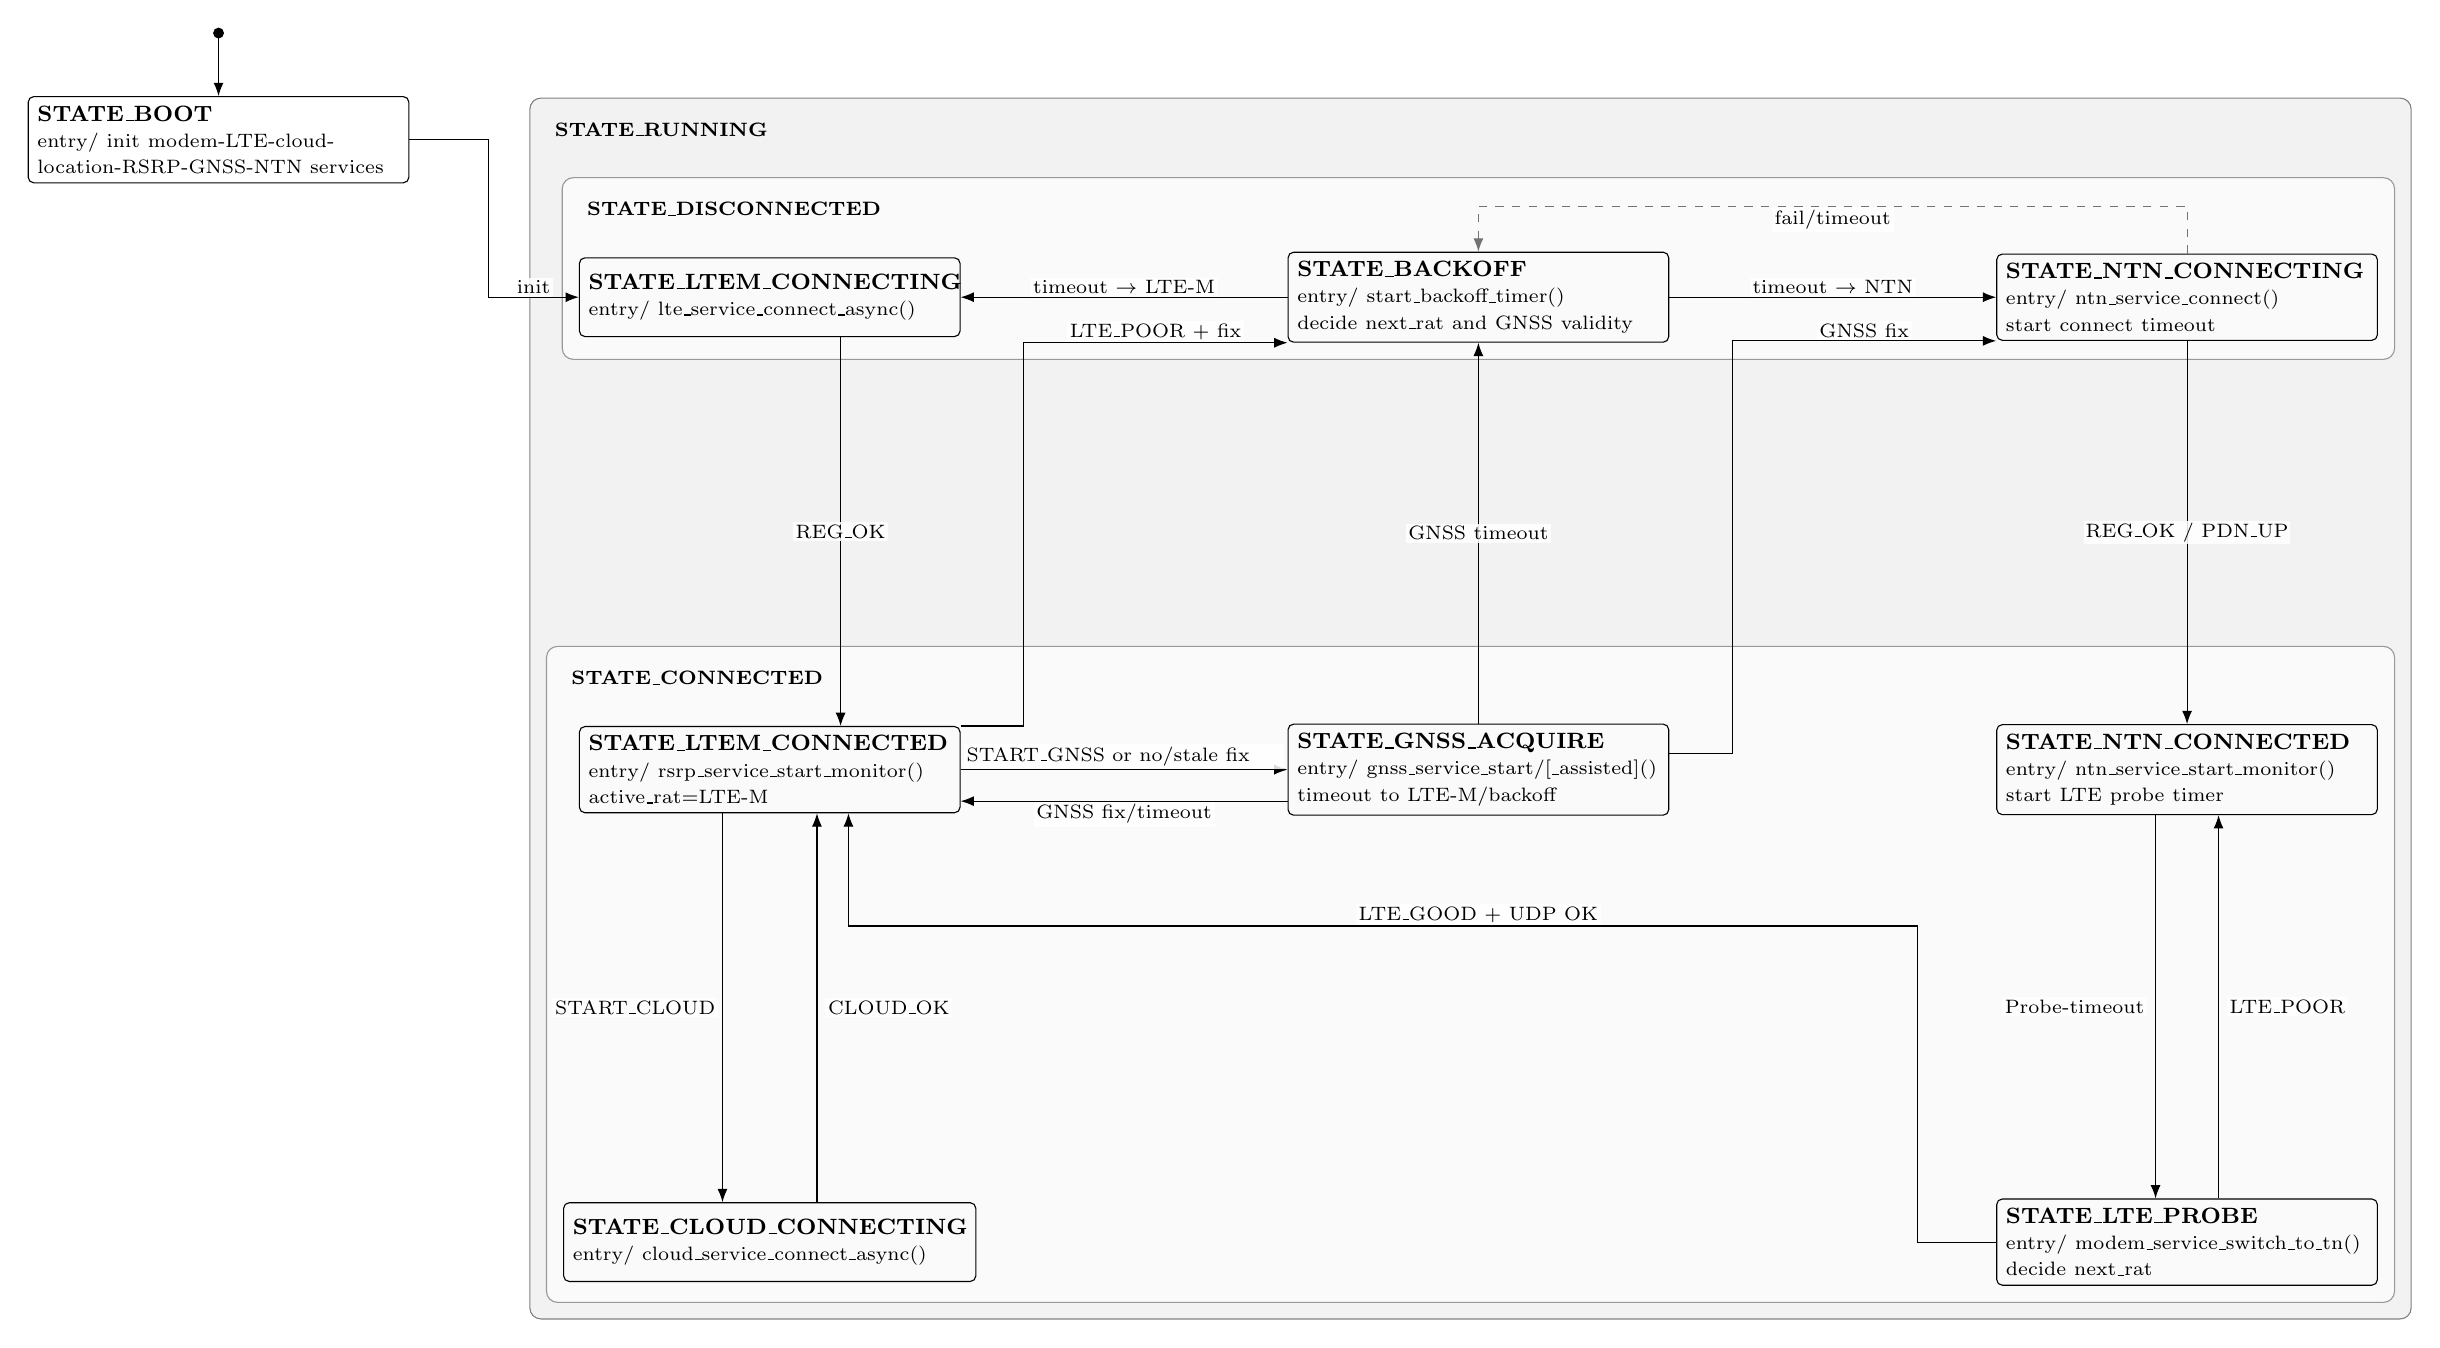
\begin{tikzpicture}[
    state/.style={process, rounded corners=2pt, align=center, text width=52mm, minimum height=8mm, font=\footnotesize},
    stateNote/.style={process, rounded corners=2pt, align=left, text width=46mm, minimum height=10mm, font=\footnotesize},
    stateSmall/.style={process, rounded corners=2pt, align=center, text width=36mm, minimum height=7mm, font=\scriptsize},
    edgeLabel/.style={font=\scriptsize, align=left, fill=white, fill opacity=0.85, text opacity=1, inner sep=1pt},
    init/.style={circle, fill=black, draw=black, inner sep=1.2pt, minimum size=3.5pt},
    containerRunning/.style={draw=black!50, rounded corners, fill=black!5, inner sep=8pt},
    containerSub/.style={draw=black!40, rounded corners, fill=black!2, inner sep=6pt},
    containerLabel/.style={font=\scriptsize\bfseries},
    lineMuted/.style={line, draw=black!55, dashed}
]

% layout grid
\def\colBoot{-7}
\def\colL{0}
\def\colM{9}
\def\colR{18}
\def\rowBoot{6}
\def\rowTop{4}
\def\rowMid{-2}
\def\rowLow{-8}
\def\rowLower{-14}

% states
\node[stateNote] (boot) at (\colBoot,\rowBoot) {
    \textbf{STATE\_BOOT}\\
    {\scriptsize entry/ init modem-LTE-cloud-location-RSRP-GNSS-NTN services}
};

\node[stateNote] (ltem_connecting) at (\colL,\rowTop) {
    \textbf{STATE\_LTEM\_CONNECTING}\\
    {\scriptsize entry/ lte\_service\_connect\_async()}
};

\node[stateNote] (backoff) at (\colM,\rowTop) {
    \textbf{STATE\_BACKOFF}\\
    {\scriptsize entry/ start\_backoff\_timer()}\\
    {\scriptsize decide next\_rat and GNSS validity}
};
\node[stateNote] (ntn_connecting) at (\colR,\rowTop) {
    \textbf{STATE\_NTN\_CONNECTING}\\
    {\scriptsize entry/ ntn\_service\_connect()}\\
    {\scriptsize start connect timeout}
};

\node[stateNote] (ltem_connected) at (\colL,\rowMid) {
    \textbf{STATE\_LTEM\_CONNECTED}\\
    {\scriptsize entry/ rsrp\_service\_start\_monitor()}\\
    {\scriptsize active\_rat=LTE-M}
};
\node[stateNote] (gnss_acquire) at (\colM,\rowMid) {
    \textbf{STATE\_GNSS\_ACQUIRE}\\
    {\scriptsize entry/ gnss\_service\_start/[\_assisted]()}\\
    {\scriptsize timeout to LTE-M/backoff}
};
\node[stateNote] (ntn_connected) at (\colR,\rowMid) {
    \textbf{STATE\_NTN\_CONNECTED}\\
    {\scriptsize entry/ ntn\_service\_start\_monitor() start LTE probe timer}
};

\node[stateNote, text width=50mm] (cloud_connecting) at (\colL,\rowLow) {
    \textbf{STATE\_CLOUD\_CONNECTING}\\
    {\scriptsize entry/ cloud\_service\_connect\_async()}
};
\node[stateNote] (lte_probe) at (\colR,\rowLow) {
    \textbf{STATE\_LTE\_PROBE}\\
    {\scriptsize entry/ modem\_service\_switch\_to\_tn()}\\
    {\scriptsize decide next\_rat}
};

% hierarchy boxes (background)
\coordinate (disconnectedHeader) at ($(ltem_connecting.north west)+(0,8mm)$);
\coordinate (connectedHeader) at ($(ltem_connected.north west)+(0,8mm)$);
\coordinate (runningHeader) at ($(disconnectedHeader)+(0,8mm)$);

\begin{scope}[on background layer]
    \node[containerRunning, inner sep=12pt] (runningBox)
        [fit=(runningHeader)(ltem_connecting)(backoff)(ntn_connecting)(ltem_connected)(gnss_acquire)(ntn_connected)(lte_probe)(cloud_connecting)] {};
    \node[containerSub] (disconnectedBox)
        [fit=(disconnectedHeader)(ltem_connecting)(backoff)(ntn_connecting)] {};
    \node[containerSub] (connectedBox)
        [fit=(connectedHeader)(ltem_connected)(gnss_acquire)(ntn_connected)(lte_probe)(cloud_connecting)] {};
\end{scope}

% parent labels inside containers
\node[containerLabel, anchor=north west] at ($(runningBox.north west)+(2mm,-2mm)$) {STATE\_RUNNING};
% STATE_RUNNING initial/default child indicator
%\node[init] (init_running) at ($(runningBox.north west)+(100mm,-4mm)$) {};

%\draw[line, rounded corners=6pt]
%    (init_running)
%    -| ([xshift=-8mm]disconnectedBox.north);

\node[containerLabel, anchor=north west] at ($(disconnectedBox.north west)+(2mm,-2mm)$) {STATE\_DISCONNECTED};
\node[containerLabel, anchor=north west] at ($(connectedBox.north west)+(2mm,-2mm)$) {STATE\_CONNECTED};

% UML initial nodes
\node[init] (init_boot) at ($(boot.north)+(0,8mm)$) {};
\draw[line] (init_boot) -- (boot.north);

% main flow
\coordinate (boot_out) at ($(boot.east)+(10mm,0)$);
\coordinate (boot_turn) at (boot_out |- ltem_connecting.west);
\coordinate (boot_label) at ($(boot_turn)!0.5!(ltem_connecting.west)$);
\draw[line] (boot.east) -- (boot_out) |- (ltem_connecting.west);
\node[edgeLabel, above] at (boot_label) {init};
\draw[line]
    ([xshift=9mm]ltem_connecting.south)
    -- node[
        edgeLabel,
        midway,
        fill=white,
        inner sep=1pt
    ] {REG\_OK}
    ([xshift=9mm]ltem_connected.north);

\draw[line] ([xshift=-6mm]ltem_connected.south) -- node[edgeLabel, left, xshift=-0.5mm]{START\_CLOUD} ([xshift=-6mm]cloud_connecting.north);
\draw[line] ([xshift=6mm]cloud_connecting.north) -- node[edgeLabel, right, xshift=1mm]{CLOUD\_OK} ([xshift=6mm]ltem_connected.south);

\draw[line] (ltem_connected.east) -- node[edgeLabel, above, text width=40mm]{START\_GNSS or no/stale fix} (gnss_acquire.west);
\draw[line] ([yshift=-4mm]gnss_acquire.west) -- node[edgeLabel, below]{GNSS fix/timeout} ([yshift=-4mm]ltem_connected.east);

% fallback path
\coordinate (ltem_backoff_out) at ($(ltem_connected.north east)+(8mm,0)$);
\coordinate (ltem_backoff_turn) at (ltem_backoff_out |- backoff.south west);
\coordinate (ltem_backoff_label) at ($(ltem_backoff_turn)!0.5!(backoff.south west)$);
\draw[line] (ltem_connected.north east) -- (ltem_backoff_out) |- (backoff.south west);
\node[edgeLabel, above] at (ltem_backoff_label) {LTE\_POOR + fix};
\draw[line]
    (gnss_acquire.north)
    -- node[
        edgeLabel,
        midway,
        fill=white,
        inner sep=1pt
    ] {GNSS timeout}
    (backoff.south);
\coordinate (gnss_ntn_out) at ($(gnss_acquire.east)+(0,2mm)$);
\coordinate (gnss_ntn_mid) at ($(gnss_ntn_out)+(8mm,0)$);
\coordinate (gnss_ntn_turn) at (gnss_ntn_mid |- ntn_connecting.south west);
\coordinate (gnss_ntn_label) at ($(gnss_ntn_turn)!0.5!(ntn_connecting.south west)$);
\draw[line] (gnss_ntn_out) -- (gnss_ntn_mid) |- (ntn_connecting.south west);
\node[edgeLabel, above] at (gnss_ntn_label) {GNSS fix};

\draw[line] (backoff.east) -- node[edgeLabel, above]{timeout $\rightarrow$ NTN} (ntn_connecting.west);
\draw[line] (backoff.west) -- node[edgeLabel, above]{timeout $\rightarrow$ LTE-M} (ltem_connecting.east);

% NTN path
\draw[line]
    (ntn_connecting.south)
    -- node[edgeLabel, midway, fill=white, inner sep=0.5pt]
    {REG\_OK / PDN\_UP}
    (ntn_connected.north);
\coordinate (ntn_fail_up) at ($(ntn_connecting.north)+(0,6mm)$);
\coordinate (backoff_fail_up) at (backoff.north |- ntn_fail_up);

\draw[lineMuted]
    (ntn_connecting.north)
    -- (ntn_fail_up)
    -- node[edgeLabel, below]{fail/timeout} (backoff_fail_up)
    -- (backoff.north);
\draw[line]
    ([xshift=-4mm]ntn_connected.south)
    -- node[edgeLabel, left, xshift=-1mm]{Probe-timeout}
    ([xshift=-4mm]lte_probe.north);

% LTE probe loop
\draw[line] ([xshift=4mm]lte_probe.north) -- node[edgeLabel, right, xshift=1mm]{LTE\_POOR} ([xshift=4mm]ntn_connected.south);
\coordinate (probe_return) at ($(gnss_acquire.south)+(0,-14mm)$);
\coordinate (probe_left) at ($(lte_probe.west)+(-10mm,0)$);
\coordinate (probe_entry) at ($(ltem_connected.south)+(10mm,0)$);
\coordinate (probe_entry_y) at (probe_entry |- probe_return);
\draw[line]
    (lte_probe.west)
    -- (probe_left)
    |- (probe_return)
    -- node[edgeLabel, above, pos=0]{LTE\_GOOD + UDP OK}
    (probe_entry_y)
    -- (probe_entry);
%\node[edgeLabel, below, align=left] (probe_note) at ($(lte_probe.south)+(0,-10mm)$) {Probe failure: reconnect LTE-M\\or return to NTN};

\end{tikzpicture}
\end{document}
